\documentclass[12pt,a4paper]{report}
\usepackage{tikz}
\usepackage{hyperref}
\usepackage{amsmath}
\usepackage{amssymb}
\usepackage{amsthm}
\usetikzlibrary{arrows,positioning}
\tikzset{ >=stealth', punkt/.style={ rectangle, rounded corners, draw=black, very thick, text width=6.5em,minimum height=2em, text centered}, pil/.style={ ->, thick, shorten <=2pt, shorten >=2pt,}}
\begin{document}
 \href{doc/jokes.html}{Previous} 
 \href{doc.html}{Up} 

 \href{doc/phil.pdf}{PDF} 
\title{phil}

\tableofcontents
Things related to philosphy.
\part{doc/phil/People.html|People}

\chapter{doc/phil/People/Brandom.html|Brandom}

\section{doc/phil/People/Brandom/Antirepresentationalism.html|Antirepresentationalism}
A lecture series taught in 2020.
\subsection{doc/phil/People/Brandom/Antirepresentationalism/Lecture01.html|Lecture01}

\subsection{doc/phil/People/Brandom/Antirepresentationalism/Lecture02.html|Lecture02}

\subsection{doc/phil/People/Brandom/Antirepresentationalism/Lecture03.html|Lecture03}

\subsection{doc/phil/People/Brandom/Antirepresentationalism/Lecture04.html|Lecture04}

\subsection{doc/phil/People/Brandom/Antirepresentationalism/Lecture05.html|Lecture05}

\subsection{doc/phil/People/Brandom/Antirepresentationalism/Lecture06.html|Lecture06}

\subsection{doc/phil/People/Brandom/Antirepresentationalism/Lecture07.html|Lecture07}

\subsection{doc/phil/People/Brandom/Antirepresentationalism/Lecture08.html|Lecture08}

\subsection{doc/phil/People/Brandom/Antirepresentationalism/Lecture09.html|Lecture09}

\subsection{doc/phil/People/Brandom/Antirepresentationalism/Lecture10.html|Lecture10}

\subsection{doc/phil/People/Brandom/Antirepresentationalism/Lecture11.html|Lecture11}

\subsection{doc/phil/People/Brandom/Antirepresentationalism/Lecture12.html|Lecture12}

\subsection{doc/phil/People/Brandom/Antirepresentationalism/Lecture13.html|Lecture13}

\subsection{doc/phil/People/Brandom/Antirepresentationalism/Lecture14.html|Lecture14}

\section{doc/phil/People/Brandom/OnSellars.html|On Sellars}
Robert Brandom taught a recorded graduate seminar on Wilfred Sellars twice, in 2009 and and 2019. Notes on the recordings of these lectures are collected here.
\subsection{doc/phil/People/Brandom/OnSellars/2009.html|2009}

\subsubsection{doc/phil/People/Brandom/OnSellars/2009/Lecture01.html|Lecture01}
The first of many lectures by Robert Brandom on Wilfred Sellars, delivered on September 2, 2009.

\paragraph{doc/phil/People/Brandom/OnSellars/2009/Lecture01/HistoricalKantContext.html|Historical Kant Context}
Kant was not in favor within analytic philosophy when Sellars began. ``One cannot open the door enough for Kant to get through while being able to slam it shut before Hegel gets through.'' (He's too interesting of a reader, and Hegel was the great bad of Anglophone philosophy). Though it's also ironic since Kant is incredibly analytical and science-driven.

Four ideas of Kant that mattered to Sellars:
\begin{enumerate}
\item \textbf{Kant's normative turn}:
\begin{itemize}
\item His normative understanding of discursive (i.e. relating to concepts) practice. Kant saw that what distinguishes judgments/intentional behavior from habitual behavior is that there are things that the agents are in a distintive sense \emph{responsible} for. this point is shared by the later Wittgenstein. The \href{doc/phil/Phil Situations/Childrens Game.html}{puzzles} that Wittgenstein offers us (along the way to trying to dissolve the presuppositions that make it puzzling) center around the normative significance of beliefs/desires/intentions.

\item The difference between us and it is not an \emph{ontological} distintion but rather a \emph{deontological} distinction. Downstream of this is many of Kant's innovations. The minimum unit of awareness/experience is the judgment (you need concepts already for that). The subjective form of judgment (the ``I think", the emptiest form of judgment) mark of "who is responsible for the judgment" vs the subjective form of judgment the mark of what you've made yourself responsible to. In virtue of having your made yourself responsible to what you say you're talking about, is what make it that you're representing (it sets the standards of correctness).
\end{itemize}

\item \textbf{Turning Rousseau's definition of freedom into demarcating the normative}: Rousseau said ``Obedience to a law that one has laid oneself is freedom''. Kant turned this around to distinguish constraint by norms from constraint by power. Where natural things are bound by rules, we are bound by our conceptions of rules (i.e. to the extent we acknowledge them). Our normative status depend on our attitudes.

\item \textbf{Pure concepts of the understanding}: In addition to concepts whose principle expressive job is to describe/explain empirical goings-on, there are concepts whose principle expressive job it is to make explicit the framework that makes description possible. These are known \textit{a priori}. Framework-explicating concepts. This is Kant's response to Hume, for how we can understand the modal force of laws in virtue of their non-modal description. The answer is in the description framework itself. The fact that there are necessarily relations that concepts have among another makes description possible (a concept being contentful at all requires it to have some necessary relations to other concepts). What Sellars means by `ushering philosphy from its Humean phase to its Kantian phase' is putting categories front and center. Trying to \emph{describe} the modal structure of the world or describe the space of possible worlds is to try to assimilate modal language into descriptivism, rather than seeing them as playing a different expressive role (Sellars saw Kant as putting this other option on the table).
\end{enumerate}. Difference between Humean thinking and Kantian thinking: do you take this categorial status in some form (rather than it being descriptive) - `laws of nature are not super-facts - you are not describing the world'. It's a transposed rule of inference.

Another Kantian idea: the distinction between phenomena and noumena. Kant radicalized the distinction between primary and secondary qualities (properties that are truly there vs properties that are due to us). He challenges us to divide the labor, what features is the world responsible for vs are we responsible for (e.g. the fact our theories are expressed in German/English)? This distinction lives in Sellars as the difference between the world (in the narrow sense) and the world (in the wider sense ... e.g. including norms that are only accessible from a participant's perspective).

\paragraph{doc/phil/People/Brandom/OnSellars/2009/Lecture01/Sellarsquotes.html|Sellars quotes}
Some Sellars quotes on Describing, explaining, and justifying.

He doesn't begin with philosophically elaborated definition of describing, explaining, justifying. He takes these concepts as they come. He wants to do philosophy in a neutral / as close-to-practice way as possible.

\subsubsection{doc/phil/People/Brandom/OnSellars/2009/Lecture02.html|Lecture02}
This lecture was delivered on September 9, 2009.This lecture was delivered on September 9, 2009.

\paragraph{doc/phil/People/Brandom/OnSellars/2009/Lecture02/SellarsStyle.html|Sellars Style}
% ORD 1
% GIST The 'mystery story' vs 'journalistic' styles of philosophical writing.

\begin{itemize}
\item `Mystery story' style:
    \begin{itemize}
        \item There's a problem, and many competing potential explanations
        \item These explanations engage each other dialectically
        \item Only at the end would you learn the philosopher's actual position
    \end{itemize}
\item `Journalistic' style:
    \begin{itemize}
        \item Tell them what you're going to tell them
        \item Tell them
        \item tell them what you told them
    \end{itemize}
\end{itemize}

Sellars philosophical style is more the former.
\paragraph{doc/phil/People/Brandom/OnSellars/2009/Lecture02/MaterialInference.html|Material Inference}
% ORD 2
% GIST An inference that is good NOT due to their logical form.
% TAG Def

Descriptive terms appear vacuously when in logically valid inferences and essentially when in \emph{material inferences}. You can turn a good material inference into a bad one by substituting some nonlogical vocabulary for different nonlogical vocabulary, but you cannot turn a logically valid inference into a bad one by the same means. Example: $P \land Q \implies P$ goes through regardless of what we substitute for $P$ and $Q$, but the material inference ``$a$ is red'' $\implies$ ``$a$ is colored'' will become false if we replace `colored' with `square'.

\paragraph{doc/phil/People/Brandom/OnSellars/2009/Lecture02/MaterialInferenceMainIdea.html|Material Inference Main Idea}
% ORD 3
% GIST Material inference a more primitive notion than logical validity.

Sellars has two good ideas associated with material inference:
\begin{enumerate}
\item There \emph{are} some inferences that are good, not in virtue of their logical form.
\item Turn the above thought on its head and say: we can understand the content of these descriptive terms in terms of the materially good inferences they appear in (as premises or conclusions).
\end{enumerate}

%Historical aside:
%This idea is connected to Bolzano (a contemporary of Frege's), who thought about how abstraction was connected to reasoning. We look at a good inference and the class of substitutions under which it remains good. This allows us to move from an equivalence relation to the equivalence class. Frege takes this and uses this as the basis for his logic and metaphysics. his notion of a function is understood in terms of substitutions / inter-substitutions.
%Quine picked up this substitution methodology in some of his technical writings (e.g. his essay on Carnap on logical truth). Quine talks about logical things as ones in which all non-logical vocabulray occurs vacuously (not in a way that's essential to the goodness of inference).

By this account, material proprieties of inference are more fundamental than / conceptually prior to logical validity. You have to start with the notion of a good inference in order to understand what a logically good inference is.

\paragraph{doc/phil/People/Brandom/OnSellars/2009/Lecture02/PhilofLogicAside.html|Phil of Logic Aside}
% ORD 4
% GIST Basic questions in philosophy of logic.

Aside: It took a while in the 20th century to realize that logic was not about
logical truth but rather about validity of inference. In classical logic can
you treat these interchangably, but not all (rough logics vs smooth logics -
whether the consequence relation can be determined by the set of all theorems).
Dummett has written about this issue.

What if we picked some other vocabulary (other than logical) to hold fixed? E.g.
substituting non-theological vocabulary for non-theological vocabulary.
``If justice is loved by the gods then justice is pious''. If no matter what we
substitute for justice the inference is good, we might say the sentence is true
in virtue of its theological form.

Philosophy of logic (See Quine's and Putnam's books both titled The Philosophy
of Logic) has two classic questions:
\begin{enumerate}
    \item a \emph{demarcation} question: what makes something logical vocabulary?
     \begin{itemize}
        \item Quine disallows second order quantifiers and the epilson of set
              theory, whereas Putnam allows them.
     \end{itemize}
    \item a \emph{correctness} question: which logical consequence relation to use:
      \begin{itemize}
      \item Classical? Intuitionistic? etc.
      \end{itemize}
\end{enumerate}

Sellars challenges this tradition (logical empiricism) by pointing out there is
a concern conceptually prior in the order of explanation to philosophy of
logic: materially good inferences.

\paragraph{doc/phil/People/Brandom/OnSellars/2009/Lecture02/InferenceandMeaning.html|Inference and Meaning}
% ORD 5

A main argument of \textit{Inference and Meaning} (cite) is that any language that makes essential use of non-logical, descriptive vocabulary must be understand as having that vocabulary standing in materially good (rather than just logically good) inferences.

``Concepts as Involving Laws and inconceivable without them'' is the title of an unintelligible essay by Sellars (but the title is the thesis and intelligible).

Sellars answers the first major question by claiming logical vocabulary (more specifically, alethic modal vocabulary, about what's necessary and what's possible) has the expressive job of making explicit the material proprieties of inference that articulate the content of non-logical concepts. Frege is more explicit about this (that you can use this to distinguish logical vocabulary) than Sellars.

Dan Dennett argues that we have to take animals as grasping modus ponens because they treat some inferences as good and others as bad (see \ref{phil-scenarios-section-dog-disjunction}). You could make explicit the practical capacity the animal has using a statement of disjunctive syllogism, but Sellars would ask what is the surplus value of invoking that explicit expression? (Over simply describing what is the dog can do).

There have to be some practical moves you're just allowed to make without them having to take the form of explicit premises (see \ref{phil-problems-section-tortoise}). Sellars touches upon this in Reflections on Language Games. He talks about free/auxillary positions that you're always allowed to occupy. We could have the auxillary position $\forall x, \psi(x)\vdash \phi(x)$ which would license us to move from a position $\psi(a)$ to a position $\phi(a)$, but we could also encode this with position for each possible move ($\psi(a)\vdash \phi(a)$, $\psi(b)\vdash\phi(b)$, ...). He ways that we could imagine replacing positions with moves, but it's not possible to imagine all moves being replaced with positions (`a game without moves is Hamlet without the Prince of Denmark').

Sellars is addressing tradition that wants some small set of explicit principles in accordance with which to reason. Any inference you think is good that isn't derivable from that small set of principles (e.g. modus ponens) is actually an infamy (has some suppressed premises). This is early analytic philosophy's embrace of the new logic. Sellar's contrary view (radical at the time) is that actually the reasoning could be completely in order, just with material proprieties of reasoning. You can still give/ask for reasons and mean that $p$, but what the logic does is give you meta-linguistic control to talk about what is a good inference and say that $p \vdash q$ is a good inference. Sellars doesn't extrapolate from this that logic is an optional superstructure in our lives - we need to be able to think and talk about the goodness of inferences.

Brandom: logic is the organ of semantic self-consciousness. The set of concepts that lets us bring our endorsement of some inferences as good/bad (this endorsement as something that reasons can be given or asked for) into the game of giving/asking for reasons.

Example: $A\vdash B$ where $A$ is ``she asked me to hand her the dish towel" and $B$ is ``I shall hand her the dish towel''. Traditional analytic philosophy will call this an infamy since it does not explicitly state how her request engages my motivational structure. Sellars would want to say that this invocation of the desire makes explicit the endorsement of $A \vdash B$ rather than referring to some item of the world.

Sellars complains about Carnap treating logical consequence as a syntactically definable relation between sentences. Just writing down the rules under a heading `rules' instead of `axioms' isn't making explicit the normative force they have (it leaves out the rulishness - that a rule is a rule for \emph{doing} something). This is a subtle point that doesn't matter for many purposes, but Sellars believes it's important if you want to understand what's going on with reasoning.

Potential counterargument against sellars: subjunctive conditionals are not making explicit proprieties of inference, but in fact are descriptions about possible worlds. To address this, we note there are separate issues. Firstly, there's the question about whether it's intelligible to have descriptive vocabulary in play in a context where there's no counterfactual reasoning. E.g. Hume believes he understands empirical facts perfectly well (the cat is on the mat) but not statements about what's possible and necessary. But Kant saw that this isn't intelligble - you need to make a distinction about what's possible with the cat and what's not (it's possible for the cat to not be on the mat, but not possible for it to be larger than the sun) or else there's nothing you could say about the conctent of the concept of `cat' that I've got (it would be just a label). The second issue is the codifiability of proprieties of material inference by logical vocabulary: whether a possible worlds analysis is incompatible with seeing subjunctive conditionals as making properties of inference explicit. Sellars would like to see a possible worlds analysis that matches up.

``There's an important difference between logical / modal / normative predicates on the one hand, and such predicates as `red' on the other.'' There's nothing to the formal except their role in reasoning, indeed, their role and make as meta linguistics sort of making explicit something about the ground level. For the latter, he wants to argue that these predicates too are meaningful insofar as their role in reasoning, but it's less obvious.

``Red is a quality''. This conveys the same information as the syntactical sentence ``\textit{Red} is a one place predicate.'' \ref{phil-quotes-section-modalities-and-norms}. What you're doing in asserting that premise from which to reason (couched in modal vocabulary) is endorsing a principle in accordance with which to reason (couched in normative vocabulary).

We cannot completely identify modal and normative statements. When I say "copper melts at 1084 degrees" one makes a claim that is true even if ther were no reasoners (so it can't be a claim directly \emph{about} inferences being good). What it \emph{conveys} is about inferences, not what it \emph{says}. Likewise, I say ``The sun is shining'' while I convey ``I believe the sun is shining.''

It might help to make progress toward understanding the say/convey distinction (which Sellars admits he's not clear about) by distinguishing two flavors of inference:
\begin{enumerate}
\item semantic inference: good in virtue of the contents of the premises and the conclusion
\item pragmatic inference: good in virtue of what you're doing in asserting the premises or the conclusion.
 \begin{itemize}
 \item e.g. John says `your book is terrible' and I infer that he's mad at me
 \item Geech embedding distinction between the two: we look at whether we'd endorse ``My book is terrible, then John is mad at me". Because we wouldn't, we know the inference is pragmatic.

 \end{itemize}
\end{enumerate}
\paragraph{doc/phil/People/Brandom/OnSellars/2009/Lecture02/SomeReflectionsonLanguageGames.html|Some Reflections on Language Games}
% ORD 7

Regulism (conceptual norms as a matter of explicit rules) vs regularism (norms in terms of actual regularities). These are identified with empiricist and rationalist approaches. (Kris: I also see prescriptivism and descriptivism in linguistics)

One purpose: ``I shall have a chief my present purpose if I've made plausible the idea that an organism might come to play a language game, that is to move from position to position, the system of moves and positions, and to do it because of the system without having to obey rules, and hence without having to be playing a meta language game.'' (Section 18)

He doesn't explicitly mention Wittgenstein (\ref{jokes-subsection-worst-philosopher}). (Other times he uses astrices to censor his name). Thinking about language in terms of rules is Kantian. His notion of norms was juridical/jurisprudential. A rule that enjoins the doing of an action A is a sentence in some language, which requires more rules to interpret (regress - how do we deal with it?). Kant identified this regress (A132/B171) - ``judgment is a peculiar talent that can be practiced only and not taught''. Which is using distinction between things that can be shown (by examples) vs taught. Wittgenstein addresses this regress in the late 100's of PI.

Rejecting mere conformity: If we just consider conforming to a rule rather than obeying a rule, there's no regress, but we lose the normativity.

``[Mere conformity people] claim that it's raining therefore the streets will be wet (when it isn't an infamatic abridgement of a formally valid argument) is merely the manifestation of a tendency to expect to see the wet streets when one finds it's raining. In this latter case, it's a manifestation of a process which at best can only simulate inference, since it's a habitual transition, and as such not governed by a principle or rule by reference to which can be characterized as valid or invalid. That Hume dignified the activation of an association with the phrase `causal inference' is about a minor flaw, they continue, in an otherwise brilliant analysis. It should, however, be immediately pointed out that before one has a right to say that what Hume calls `causal inference' really is an inference at all, but merely a habitual transition from one thought to another. And contrast that with in this context, the genuine logical inferences which are, one must pay the price of showing just how logical inference is something more than a mere habitual transition empiricists in the human tradition have rarely paid this price, a fact which is proved most unfortunate for the following reason. An examination of the history of the subject shows that those who have held that causal inference only simulates inference proper have been led to do so as a result of the conviction that if it were a genuine inference, the laws of nature, things that govern this would be discovered to us by pure reason.  As they're thinking of what's a good inference having to be something that's transparent merely by introspection in the way that the laws of logic are.'' (him making point about distinction of real inferences and mere associations. )

No distinction between correct and incorrect can be made by purely pointing to regularity - as Wittgenstein pointed out, you'll always find some regularity (there's some elegant rule that generates the sequence, for any arbitrary sequence). This is also called `disjunctiv-itis' or `gerrymandering objections'. After a debate between Dretsky and Fodor: we're trying to see what makes the word porcupine mean porcupine. When `porcupine' is used in an observational way, it's typically in response to porcupines. So can we use that regularity to understand what `porcupine' means? No, because of counterfactuals. If it happened that the porcupines we saw were almost always male, would the word mean male porcupine? Or if we look at dispositions, if they're disposed to also call echidnas porcupines (that's the disjunction), why not say that `porcupine' means porcupine or echidna?

``what's denied is the playing a game logically involves obedience to the rules of the game. And hence the ability to use the language to play the language game in which the rules are formulated.'' (page 29) Need a sense of playing the game stronger than conforming but weaker than having the rules in mind.

Metaphysicus suggests why not a non-linguistic awareness of the rules? This is its own regress.

``We've tacitly accepted so far and the dialectic dichotomy between merely conforming to the rules and obey. But surely this is a false dichotomy. Is there something in between, for it required us to suppose that the only way in which a complex system of activity can be involved in the explanation of the occurrence of a particular act is by the agent explicitly envisaging the system and intending its realization. And that's as much as to say that unless the agent conceives of the system, the conformity of his behavior to the system must be accidental. '' So what's needed he's saying, is going to be something that says, look, there's an explanation of why he conforms to the rules. That invokes the rules, but it doesn't invoke them by him being aware of them. One example of this is teleosemantics \ref{phil-situations-section-bee-waggles}.

The essential thing for Kant was a distinction between what was between acting according to a rule and acting according to a conception of a rule, or a representation (Vorstellung) of a rule. So, ordinary natural objects act according to rules, the laws of nature, but we act according to representations of rules / to conceptions of rules.

The explanation as to why I use the word `purple' for purple things, the rule plays a crucial part even if it is not in my head. It is in the teachers' heads (they're already in the language and can conceive of rules). So the rule is causally antecedent to my behavior, so I can be following the rule (without regress).

Related quesiton addressed here: \ref{phil-situations-section-classical-behaviorism}

How is it that I can apply a concept according to norms, to invoke a pre-linguistic awareness of universals, that's going to be a given. And the key thing is, because that pre-linguistic awareness is conceived of as providing \emph{reasons} for me to do this. It's not just that I've been \emph{trained} to respond to some physiological thing by doing it (that would be okay. That could be part of the the real explanation, the pattern governed explanation). It's that that pre-linguistic awareness provides reasons. And the claim is reasons are always making a move in a game that's making the inferential move. And the question is: what determines the norms that govern that? Then we're off on the on the regress, again, so we've got to have some story that doesn't have that form. The form of the argument against the myth of the given. It's the idea that the awareness that givenness provides something that can serve as a reason, but is itself not dependent on our having learned a language, having a conceptual scheme, and so on.

To do: understand language entry transitions and language exit transitions.

There is debate (but it should be more of a bigger deal, in Brandom's opinion) about what are the minimal features needed for one to have a discursive language practice. Brandom views logical language as optional (though the expressive power would be incredibly stunted, you could still give and ask for reasons). MacDowell and Sellars think otherwise, that there can't be discourse without a meta-language.

Sellars needs the notion of language to be something that evolves over time (rather than an instantaneous collection of rules) because we want the decision to make a material move to occur with in a language (one is not doing redescription in another language).
\subsubsection{doc/phil/People/Brandom/OnSellars/2009/Lecture03.html|Lecture03}
This lecture was delivered on September 16, 2009.

\subsubsection{doc/phil/People/Brandom/OnSellars/2009/Lecture04.html|Lecture04}
This lecture was delivered on September 23, 2009.

\subsubsection{doc/phil/People/Brandom/OnSellars/2009/Lecture05.html|Lecture05}
This lecture was delivered on September 30, 2009.

\subsubsection{doc/phil/People/Brandom/OnSellars/2009/Lecture06.html|Lecture06}
This lecture was delivered on October 7, 2009.

\subsubsection{doc/phil/People/Brandom/OnSellars/2009/Lecture07.html|Lecture07}
This lecture was delivered on October 14, 2009.

\subsubsection{doc/phil/People/Brandom/OnSellars/2009/Lecture08.html|Lecture08}
This lecture was delivered on October 21, 2009.

\subsubsection{doc/phil/People/Brandom/OnSellars/2009/Lecture09.html|Lecture09}
This lecture was delivered on October 28, 2009.

\subsubsection{doc/phil/People/Brandom/OnSellars/2009/Lecture10.html|Lecture10}
This lecture was delivered on November 11, 2009.

\subsubsection{doc/phil/People/Brandom/OnSellars/2009/Lecture11.html|Lecture11}
This lecture was delivered on November 18, 2009.

\subsubsection{doc/phil/People/Brandom/OnSellars/2009/Lecture12.html|Lecture12}
This lecture was delivered on December 2, 2009.

\subsection{doc/phil/People/Brandom/OnSellars/2019.html|2019}

\subsubsection{doc/phil/People/Brandom/OnSellars/2019/AlethicModalityI.html|Alethic Modality I}
This lecture was delivered on October 16, 2019.

\subsubsection{doc/phil/People/Brandom/OnSellars/2019/AlethicModalityII.html|Alethic Modality II}
This lecture was delivered on October 23, 2019.

\subsubsection{doc/phil/People/Brandom/OnSellars/2019/BeingandBeingKnown.html|Being and Being Known}
This lecture was delivered in late November, 2019.

\subsubsection{doc/phil/People/Brandom/OnSellars/2019/Conclusion.html|Conclusion}
This lecture was delivered on December 4, 2019.

\subsubsection{doc/phil/People/Brandom/OnSellars/2019/EPMandPhenomenalism.html|EPM and Phenomenalism}
This lecture was delivered on October 9, 2019.

\subsubsection{doc/phil/People/Brandom/OnSellars/2019/EarlyWritingsI.html|Early Writings I}
This lecture was delivered on September 04, 2019.

\paragraph{doc/phil/People/Brandom/OnSellars/2019/EarlyWritingsI/Lecture.html|Lecture}

Three historical currents:

England: Bertrand Russell and GE Moore. Introducing analytic philosophy against absolute idealism (championed by Bradley, who was influenced by Hegel-inspired T.H. Greene who was reacting negatively to dominant British empiricists). Sellars admired On Denoting.

American: At turn of the century, German idealism dominated (Josiah Royce more popular speaker than Williams James). Two movements recoiling against this: American pragmatism and "new realism/critical realism" (AKA trinonminalists, including Sellars' father, which lost to pragmatism and logical empiricism).

German/Austrian: Marbourg (natural science focus of Kant) -> Carnap + Vienna Circle. Three periods, Aufbau (radical reductive empiricism: all statements must be definable in terms of immediate experience + logical vocabulary). Carnap then lightens up (in response to CI Lewis) and says statements must at least be able to be supported by evidence that comes from experience (replacing biconditional EXPERIENCE<->THEORETICAL with just a conditional EXPERIENCE->THEORETICAL;' there's a surplus on the theoretical side).
In parallel, Frankfurt school (Adorono/Walter Benjamin/Habermas), concerned with culture (and with Marxist inflection).

Tools of the syntactical phase of logical empiricism not adequate to address all general philosophical problems - it was improved by the semantic dimensions. He wants to turn the crank again to add a pragmatic dimension.

What did Sellars see of value in the reductivist Carnap? Carnap quote: ``A symbol is introduced (or, if it is already in use, is subsequently legitimized) by determining under what conditions it is to be employed in the representation of a state of affairs. The introduction or legitimization of the word 'horse', for instance, comes about by determining the conditions which must hold if we're to call something a horse, hence through statement of the distinguishing features of a horse or the definition of horse. We say of the symbol (that has been introduced / legitimized in such a way that we think is at least capable of legitimization) that it designates a concept. So, the symbol of a concept is a rule-governed symbol. Whether it be defined or not. Its use should above all be rule-governed. The symbol should not be employed in any old arbitrary way, but rather, in a determinate consistent way. Uniformity in the mode of employemnet can be secured either by explicitly laying down rules or merely through constant habit, linguistic usage. We have not yet said anything about what a concept is, but only for what it is for a symbol to designated a concept and this is all that can be said with any precision. But it's also enough, for when talk of concepts is meaningful, it invariably addresses concepts designated by symbols or concepts that can in principle be so designated. And such talk is basically alaways about these symbols and the laws of their use. The formation of a concept consists in the establishment of the law concerning the use of the symbol it is a word in the representation in a state of affairs''. Link to sellars quote: ``Grasp of a concept is always mastery of the use of a word" Even in the Aufbau, Carnap thinks of rule-governedness of symbols being crucial to the meaning of concepts.

One way to understand the core program of analytical philosophy: the project of elaborating the meanings of a puzzling vocabulary in terms of a base vocabulary (unproblematic) with logical vocabulary. Naturalism (trying to describe intensions/norms in terms of natural science)/empiricism (trying to describe laws in terms of sense experience) as an example. (Kris: is ordinary language philosophy an example?) If it's not possible to elaborate, then the vocabulary is seens as defective in some way.

Brandom tries to synthesize this view with pragmatism as exemplified by Wittgenstein/Sellars.
\subsubsection{doc/phil/People/Brandom/OnSellars/2019/EarlyWritingsII.html|Early Writings II}
This lecture was delivered on September 11, 2019.

\subsubsection{doc/phil/People/Brandom/OnSellars/2019/EmpiricismandthePhilosophyofMind.html|Empiricism and the Philosophy of Mind}
This lecture was delivered on October 2, 2019.

\subsubsection{doc/phil/People/Brandom/OnSellars/2019/InferentialismandNormativity.html|Inferentialism and Normativity}
This lecture was delivered on September 25, 2019.

\subsubsection{doc/phil/People/Brandom/OnSellars/2019/Introduction.html|Introduction}
This lecture was delivered on August 28, 2019.

\subsubsection{doc/phil/People/Brandom/OnSellars/2019/NominalismI.html|Nominalism I}
This lecture was delivered on October 30, 2019.

\subsubsection{doc/phil/People/Brandom/OnSellars/2019/NominalismII.html|Nominalism II}
This lecture was delivered on November 5, 2019.

\subsubsection{doc/phil/People/Brandom/OnSellars/2019/PurePragmatics.html|Pure Pragmatics}
This lecture was delivered on September 16, 2019.

\subsubsection{doc/phil/People/Brandom/OnSellars/2019/ScientificRealism.html|Scientific Realism}
This lecture was delivered on November 13, 2019.

\chapter{doc/phil/People/Kant.html|Kant}

\section{doc/phil/People/Kant/Quotes.html|Quotes}

\subsection{doc/phil/People/Kant/Quotes/OnLocke.html|On Locke}
Locke (i.e. empiricism) offered ``a mere physiology of the understanding''.

Brandom repeats this a lot - what's the quote from?
\chapter{doc/phil/People/Sellars.html|Sellars}

\section{doc/phil/People/Sellars/Quotes.html|Quotes}

\subsection{doc/phil/People/Sellars/Quotes/Againstphenomenalism.html|Against phenomenalism}
``To claim that the relationship between the framework of sense contents and
that of physical objects can be construed on the phenomalist model (NB: to
think of physical objects as constellations of sense contents) is to commit
oneself to the idea that there are inductively confirmable generalizations (NB:
 subjunctive conditionals) about sense contents which are in principle capable
 of being formulated without the language of physical things. This idea is a
 mistake.'' (phenomenalism)

\subsection{doc/phil/People/Sellars/Quotes/Community.html|Community}
``To say that a person desired to do A, thought it his duty to do B, but was forced to do C, is not to describe him as one might describe a scientific specimin. One does indeed describe him, but one does something more. And it's this `something more' which is the irreducible core of the framework of persons. In what does this `something more' consist? To think of a featherless bird as a person is to think of it as a being with which  one is bound up in a network of duties. From this point of view, the irreducibility of the personal is the irreducibility of the \emph{ought} or the \emph{is}. But even more basic than this to think of a featherless biped as a person is to construe its behavior in terms of actual or potential membership in an embracing group, each member of which thinks of itself as a member of the group. Let's call such a group a \emph{community}."

Deep connection between the normative, the social, and the self-conscious.
\subsection{doc/phil/People/Sellars/Quotes/Describingandexplaining.html|Describing and explaining}
``Although describing and explaining are distinguishable, they are also in an
important sense inseparable. The descripitive and explanatory resources of
language advance hand-in-hand."

\begin{itemize}
    \item  These two kinds of discursive activity, one can be describing in a
           particular act and not explaining (and vice-versa).
    \item Globally, they're only intelligible in terms of their relation to
          each other.
    \item The claim that matters: you couldn't have an  (autonomous discursive)
          language in use that had one and not the other.
    \item The reason is at least that in order to describe something you have
          to place it in a space of implications (i.e. the above quote)
\end{itemize}
\subsection{doc/phil/People/Sellars/Quotes/Describingtheworldwithoutmodality.html|Describing the world without modality}
``The idea that the world can in principle be so described that the description
contains no modal expressions is of a piece with the idea that world can in
principle be so described such that the description contains no prescriptive
expressions.'' CDCM.

\begin{itemize}
    \item He doesn't explicitly say whether it's a bad idea or not.
    \item He wants to say modal expressions and normative expression belong in
          a box.
\end{itemize}
\subsection{doc/phil/People/Sellars/Quotes/Exemplification.html|Exemplification}
``Exemplification is a quasi-semantical relation, and it (and universals
\footnote{redness, lionhood}) is in the world only in that broad sense in which the
world includes linguistic norms and roles viewed from the standpoint of a
fellow paritipant."

\begin{itemize}
    \item This plays off Carnap's notion of `quasi-syntactical'.
    \item There's the narrow view of `the world', that's the world that science
          is the measure of all things. And the broader view of the world.
\end{itemize}

\subsection{doc/phil/People/Sellars/Quotes/Issemanticspsychological.html|Is semantics psychological}
``The means of semantical statements is no more a psychological word than is
the ought of ethical statements or the must of modal statements."

I think of this in the following way: the $\square$ operator can be applied to
statements to make them `modal' (which could be alethic, deontic, or many other
things like ``Jones thinks that ..."). One such $\square$ is ``Semantically,
...'' (or, ``Literally, ...''). Ordinary statements made in practical life
 could be interpreted as having an implicit ``Pragmatically, ...'' (in fact,
 could we define \emph{pragmatics} to be that which play this role?)
\subsection{doc/phil/People/Sellars/Quotes/Judgmentintheorderofexplanation.html|Judgment in the order of explanation}

``Kant was on the right track when he insisted that, just as concepts are
essentially (not accidentally) items which can occur in judgments, so judgments
(and therefore indirectly concepts) are items that occur essentially (not
accidentally) that occur in reasonings or arguments."

Turns a tradition (order of explanation: concepts -> judgments -> inferences)
on its head.

\subsection{doc/phil/People/Sellars/Quotes/LabelingvsDescribing.html|Labeling vs Describing}
``It's only because the expressions in terms of which we describe objects locate
them in a space of implications that they \emph{describe} at all, rather than
merely \emph{label}."

\begin{itemize}
    \item Describing is what science is the measure of all things about.
    \item You can't do everything with just classification. It's not a rich
         enough concept to get you to descriptions.
\end{itemize}
\subsection{doc/phil/People/Sellars/Quotes/Manasrationalanimal.html|Man as rational animal}
``To say that man is a rational animal is to say that man is a creature not of
habits but of rules. When God created Atom he whispered in his ear `In all
contexts of action you will recognize rules, if only the rule to grope for rules
to recognize. when you cease to recognize rules you will walk on four feet.' ''

\subsection{doc/phil/People/Sellars/Quotes/Modalexpressionsasexplanations.html|Modal expressions as explanations}
``To make firsthand use of modal expressions / subjunctive conditionals, is to
be about the business of explaining a state of affairs or justifying an
assertion." (cite CDCM).

Note we explain an (actual) state of affairs. We justify an assertion
(non-actual, in the space of reasons).

\subsection{doc/phil/People/Sellars/Quotes/Modalitiesandnorms.html|Modalities and norms}
``The language of modalities is a transposed language of norms.''

%(Related to \ref{phil-quotes-section-describing-world-without-modality})

What is the connection between the (alethic) modal sense of \emph{must} and the
 normative sense of \emph{must}.

Carnap uses `transposed' to talk about an unquoted word used in a sentence as a
transposed mode of speech (about use of a quoted-word). E.g. ``Red is a
quality.'' vs `` `Red' is a one-place predicate.''

\subsection{doc/phil/People/Sellars/Quotes/Nondescriptiveconcepts.html|Nondescriptive concepts}
``Once the tautology `the world is described by descriptive concepts' is freed
from the idea that the business of all non-logical concepts is to describe, the
 way is clear to an ungrudging recognition that many expressions which
 empiricists have relegated to second-class citizenship in discourse are not
 inferior, they're just different."

\begin{itemize}
    \item \emph{Descriptive} concepts are not the only kinds of concepts. There
         is a temptation of empiricists in assimilating all expressions to
         descriptive expressions (such that anything not intelligible as
         descriptive is defective).
    \item The negation of this is called \emph{decriptivism}.
    \item The Tractatus was supremely descriptivist, yet made a key advance by
        noting that logical expressions play a different kind of role (prior to
        Tractatus, Russell would be looking into the world to try to see what
        distinguishes positive from negative facts, when he should not have
        been looking to the world).
    \item Sellars extends this even further. The later Wittgenstein saw
        language as playing an unsurveyable variety of roles.
    \item Most interesting philosophical concepts come with a ``-ing'' ``-ed''
        distinction that's crucial. Is a justification an act of justifying vs
        what's justified (related Agrippean trilemma). Is an experience an act
        of experiencing vs what's experienced.
\end{itemize}
\subsection{doc/phil/People/Sellars/Quotes/Rulesarelived.html|Rules are lived}
``A rule, properly speaking, isn't a rule unless it lives in behavior,
rule-regulated behavior. Even rule-violating behavior. Linguistically we always
operate within a framework of living rules. To talk \emph{about} rules is to
move outside the talked about rules into another framework of living rules. The
snake which sheds its skin lives within another. In attempting to grasp rules as
rules from without, we are trying to have our cake and eat it. To describe rules
is to describe the skeletons of rules. The rule is lived, not described."
(cite LRB)

You can't be inside the rules and outside talking about them at the same time.

\subsection{doc/phil/People/Sellars/Quotes/ScientiumMensura.html|Scientium Mensura}
"In the dimension of describing and explaining the world, science is the measure
of all of things. Of what is that it is, and of what is not that it is not"

\cite{sellars1956empiricism}

\begin{itemize}
    \item The opening qualification is important but usually left out.
\end{itemize}

\subsection{doc/phil/People/Sellars/Quotes/SpaceofReasons.html|Space of Reasons}
``In characterizing an episode or a state as \emph{knowing}, we are not giving an empirical description of it. We are placing it in the logical space of reasons, of justifying and being able to justify what one says." \cite{sellars1956empiricism}
    \begin{itemize}
        \item Note, there's nothing too special about \emph{knowing}. He could also have said \emph{believing}.
        \item  We're \emph{doing} something, an act that's not \emph{describing} something.
        \item Relates to the scientium mensure quote - we have an example of something (describing knowledge) as something that science is not the measure of all things about.
        \item Rorty characterized Sellars readership as "right wing" (ones who felt the greatest philosophical illumination from ``scientium mensura") vs "left wing" (who rally behind the ``space of reasons").
        \item The Vienna circle, too, had two wings (the naturalist wing (Neurath) and the empiricist wing (Schlict)) in tension (e.g. empiricists making sense of modal statements). Carnap struggled to hold them together.
        \item Joke: Rorty says ``I hope the left and right wing Sellarsians can sort their differences out in the end more peacefully than the left and right wing Hegelians did, who settled it once and for all at a 6 month seminar called The Battle of Stalingrad.''
    \end{itemize}
\subsection{doc/phil/People/Sellars/Quotes/Subjunctiveconditionalsasessential.html|Subjunctive conditionals as essential}
``We've established not only that subjunctive conditionals are the expressions of material rules of inference, but that the authority of those rules is not derivative from formal rules. In other words, we've shown that material rules of inference are essential to the language we speak, for we make constant use of subjunctive conditions. It's very tempting to conclude that material rules of inference are essential to languages containing descriptive terms."

\subsection{doc/phil/People/Sellars/Quotes/Transitiontoconceptualthinking.html|Transition to conceptual thinking}
``Anything which can properly be called `conceptual thinking' can occur only within a framework of conceptual thinking in terms of which it can be critized, supported, refuted (in short, evaluated). To be able to think is to be able to measure one's thoughts by standards of correctness, of relevance, of evidence (NB: in the space of justification). In this sense the diversified conceptual framework is a whole which (however sketchy) is prior to its parts, and cannot be construed as a coming to gether of parts which are conceptual in character. The conclusion is difficult to avoid that the transition from preconceptual patterns of behavior to conceptual thinking is a holistic one, a jump to a level of awareness that is irreducibly new. A jump which was the coming of the being of man." - Constrast with Wittegnsteining image of ``light dawning slowly on the whole". Sellars is worried about the mechanism of how this happens.

\part{doc/phil/PhilProblems.html|Phil Problems}
This chapter is a collection of situations that are brought up as problems to be solved by various philosophers.

\chapter{doc/phil/PhilProblems/AgrippanTrilemma.html|Agrippan Trilemma}
There are only three ways of completing a proof:
\begin{itemize}
    \item The \emph{circular} argument, in which the proof of some proposition presupposes the truth of that very proposition
    \item The \emph{regressive} argument, in which each proof requires a further proof, ad infinitum
    \item The \emph{dogmatic} argument, which rests on accepted precepts which are merely asserted rather than defended
\end{itemize}

This is a dilemma for classical logic in particular; it could be addressed by introducing nonmonotonic logic (default and challenge). Some claims (e.g. first person observations) come with a default justification (which is not based on the justification of other claims). Yet it must be defended when challenged.
\chapter{doc/phil/PhilProblems/BradleysProblem.html|Bradleys Problem}
Suppose there is a relation. There is an additional relation between the relation itself and the relata. Vicious regress.

\chapter{doc/phil/PhilProblems/Universals.html|Universals}
It seems there is no problem thinking about what triangles and white things are, but what of triangularity and whiteness?

My thoughts: This seems to be an instance of the \href{doc/phil/PhilSituations/ToothPain}{tooth pain} issue. Noun-ness was for ordinary objects (with obvious ontological status) in an earlier game, but our creativity with language led us to nounify many other words, leading to `objects' with unclear ontological status.
\chapter{doc/phil/PhilProblems/WhattheTortoiseSaidtoAchilles.html|What the Tortoise Said to Achilles}

Lewis Caroll (1895)

Tortoise assumes $p$ and the conditional $p \implies q$, and Achilles tries to convince the Tortoise to accept $q$. He says that logic \emph{obliges} you to acknowledge $q$ in this case. Tortoise is willing to go along with this but demands that this rule be made explicit, so Achilles add an extra axiom $p \land (p \implies q) \implies q$. Achilles says that, now, you \emph{really} have to accept $q$ that we've written down $p$, $p \implies q$ and $p \land (p \implies q) \implies q$. But the Tortoise notes that, if that's really something logic obliges me to do, then it bears writing down ($p \land (p \implies q) \land (p \land (p \implies q) \implies q)$). Ad infinitum.

The most influential pragmatist work in the philosophy of logic, according to Brandom. The lesson: in any particular case, you can substitute a rule (that tells you you can go from this to that) with an axiom. But there have got to be some moves you can make without having to explicitly license them by a principle.  You've got to distinguish between 1.) premises from which to reason and 2.) principles in accordance with which to reason. This teaches an un-get-over-able lesson about the necessity for an implicit practical background of making some moves that are just okay. Things that would be put in a logical system, not in the forms of axioms, but in the form of rules.
\part{doc/phil/PhilSituations.html|Phil Situations}

\chapter{doc/phil/PhilSituations/BeeWaggle.html|Bee Waggle}
When a foraging bee discovers a supply of food, it returns to the hive and does
a waggle dance. The rest of the hive then flies out in a certain direction and
distance to locate the food. In some sense, the bee communicates the information
of the food supply to the hive.

Can't we explain why a particular bee on one
occasion does that by invoking the pattern that
it's an instance of? What would it mean to say of
a bee returning from a food source that it's
turnings and wiggling has occurred \emph{because}
they're part of a complete dance? This is related
to distinction of pattern governed vs rule
obeying behavior. (cite some reflections on
language games) Ruth milliken, Sellars student,
devotes her career to this, developing the field
of teleosemantics and writing about it in
Language, Thought, and Other Biological
Categories.

A simpler example than the bee one for this is
that beavers slap their tail when there's danger
and beavers flee when they hear another beaver
slap its tail.

The idea of teleosemantics is an evolutionary
sort of semantics. Acknowledge language use is
normative (make distinction between correct and
incorrect use). You have to draw the distinction
in the way that's compatible with any degree of
badness of the participants actually following
the rules. We look at a reproductive family, the
normal explanation (a tehcnial term) of tail
slapping is that, in the evolutionary history,
lives were saved by it. When the explanation of
the persistence of tail slapping turns on
particular eventsi n the past where things worked
well that way (expressed in terms of
counterfactuals - no tail slap, then species dies
out), then we can say its part of the proper
function (technical term) to perform that
behavior. This  solves some puzzle cases: it
allows us to say the proper function of sperm is
to fertilize eggs even if a vanishingly small
fraction of them actually do (because if they
hadn't fertilized eggs in the past, there
wouldn't be sperm now).

Well, this is the form of explanation for semantics, not a beaver tail slaps
that aren't involved in more complicated interactions than that. Because the
same thing can happen when the reproductive families are uses of words. Where
you can explain why, you know, we use the word Aristotle, as we do, if has
having a proper function of, in the end, referring to Aristotle, because if
people in the past had not used it, in particular ways, we wouldn't be using
it today. And similarly, for predicates, and so on. She says, These are not
biological norms. But we can understand words as having proper functions in the
same sense in which even in the merely biological case, we can understand things
as having proper functions. And we can understand them as having proper
signaling functions. So there's a proper function for producing these things
and a proper function for receiving them. There, the analogy of the of the tail
slaps is a good one.

But in order to get semantic cut to understand semantic content, we don't need
to use any principles of explanation that aren't already intelligible


\chapter{doc/phil/PhilSituations/ChildrensGame.html|Childrens Game}

A mother lets me watch her kids and says to me: Show the children a game. When she returns, she sees me teaching them to gamble with
dice. She angrily exclaims I didn't mean that sort of game! Must the exclusion
of the game with dice have come before his mind when he gave me the order?

It's true that she did mean not that sort of game. but she need not have had the conscious thought at the time of the request. Somehow her request made a normative division of proper responses.

If you find this puzzling that, nonetheless, what you did was an inappropriate response to her request, then you are trapped in a possibly Cartesian trap. You're missing what distinguishes a sign from a piece of wood.

From: \cite{wittgenstein2010philosophical}

Frac $\frac{a}{b}$!

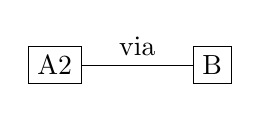
\begin{tikzpicture}
  \path (0,0) node[draw] (A) {A2};
  \path (2,0) node[draw] (B) {B};
  \draw (A) -- (B) node[midway,above = 0 em] {via};
\end{tikzpicture}


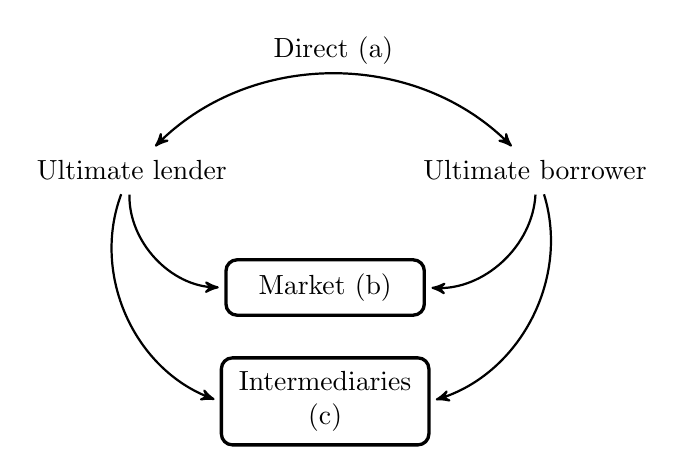
\begin{tikzpicture}[node distance=1cm, auto,]
    %nodes
    \node[punkt] (market) {Market (b)};
    \node[punkt, inner sep=5pt,below=0.5cm of market]
    (formidler) {Intermediaries (c)};
    % We make a dummy figure to make everything look nice.
    \node[above=of market] (dummy) {};
    \node[right=of dummy] (t) {Ultimate borrower}
      edge[pil,bend left=45] (market.east) % edges are used to connect two nodes
      edge[pil, bend left=45] (formidler.east); % .east since we want
                                                % consistent style
    \node[left=of dummy] (g) {Ultimate lender}
      edge[pil, bend right=45] (market.west)
      edge[pil, bend right=45] (formidler.west)
      edge[pil,<->, bend left=45] node[auto] {Direct (a)} (t);
   \end{tikzpicture}

   \vspace{1em}
   \emph{Inspired by figure 1.1 in ``Financial Markets and Institutions'' 5E
     by Howells and Bain.}



\chapter{doc/phil/PhilSituations/ClassicalBehaviorism.html|Classical Behaviorism}
This is related to the problem of: suppose you follow a rule. You use a
representation of that rule to train the next generation to follow the rule.
How do we know that the same rule is being passed on? Isn't it like a game of
telephone, given the ambiguity of following rules (gerrymandering problem - you
have a rule in your head and punish me for lifting the glass of water, but I
interpret this as punishment for lifting my arm or one of a million other
possible explanations). Brandom's response:

Well, maybe so and maybe it a given rule isn't as stable as we think. I mean,
it's only if it had enough coherence and enough stability, that we're here.
(Anthropomorphic principle). And when Wittgenstein harps on this, you know, unless
as a matter of fact, we tended to go on the same way when trained the same way,
to a remarkable extent, we wouldn't get a language game off the ground.

I should mention that this gerrymandering issue is what was wrong with classical behaviorism from an empirical point of
view. \footnote{What was wrong with
classical behaviorism, from a \emph{conceptual} point of view, is we can see it with
the wisdom of hindsight is just a larval stage on the way to functionalism. As
all of the considerations that lead people to think have direct stimulus
response connections, are satisfied still, if you allow intervening states. It's still an empirical undertaking, and so on. But there's a
lot more formal power, you can get Turing machines, if you can get functional
states, so you can get a lot farther. That's why
nobody should be a classical behaviorist anymore: be a functionalist, you get
all the advantages, and a lot more expressive power.} Remember, the stimulus and response were supposed to be
objective features of the critters you were looking at. So that the behavioral
scientist modeled on the natural scientist, her own conceptual scheme was not
supposed to be involved in characterizing the behavior of these critters. But
if you ask sort of classical studies, so I take the rat, and set him down four
steps away from the bar, and train him, then if he walks four steps forward and
presses down on the bar, he'll get a rat yummy. And that stimulus, let's say,
the light goes on, walks, four steps, pushes down on the bar gets a rat yummy.
We indoctrinate him with that, conditioned learning, he can do that. And now
we ask the behavioral scientist. And now if I put in eight steps away from
the bar, what do you predict he's going to do? Is he going to go four steps
forward and move his paw up and down? Is that the behavior that has been
associated with the stimulus? Or would you predict that he'll go eight steps
forward and press down on the bar. That is, the right description is that he'll
go from where he is to the bar and press on the bar? Well, the minute you think
about this, you realize that we can gerrymander, what he was taught,
there are many descriptions, that that are available to us for what he was
taught. And in fact, no one who works with the animals would expect him to
move four steps forward, and not be pressing on the bar. But why
is that? Is that something that you without importing any understanding of
this are objectively reading off of the situation? Or have you, in fact, all
along been importing, your characterization of what the regularity
is that you are, that you're characterizing? This is actually empirical as well a methodological
problem. What is the prediction that you're supposed to make at this point?
And how do you justify the one rather than rather than the other by your
methodological lights?

\chapter{doc/phil/PhilSituations/MontaigneDog.html|Montaigne Dog}
Montaigne is impressed that his dog, when chasing
a rabbit and coming to a fork, runs a little way
down one of the paths and smells no rabbit, then
immediately runs down the other fork of the path
without stopping to smell to check if the rabbit
went that way. (CITE?)

The dog is acting in accordance with the
disjunctive syllogism. Do we say that the dog
understands disjunction?
\chapter{doc/phil/PhilSituations/ToothPain.html|Tooth Pain}
Imagine a community that talked about having gold or silver in one’s teeth,
and extends that practice to talk about having pain in one’s teeth. If, as a
matter of contingent fact, the practitioners can learn to use the expression
‘in’ in the new way, building on (but adapting) the old, they will have
fundamentally changed the \emph{meaning} of ``in". This can be seen by the
fact that, in the old practice, it made sense to ask where the gold was before
it was in one’s tooth, whereas in the new practice asking where the pain was
before it was in the tooth can lead only to a distinctively philosophical kind
of puzzlement.

\cite{brandom2019some}

\bibliography{my}
\bibliographystyle{amsalpha}
\end{document}